Per quanto riguarda invece la rete neurale incaricata al riconoscimento delle pupille, viene creata e addestrata in maniera simile alla nostra prima rete neurale. In questa fase ci limitiamo a crearla, in un secondo momento, durante l'implementazione Android, essa userà come input l'output della prima rete neurale dedicata agli occhi.

\subsection{Dataset}
\label{sub:gazedataset}
Per il training del modello si è utilizzato un dataset pubblico rilasciato da Google\footnote{Open Image V6, \url{https://storage.googleapis.com/openimages/web/index.html?v6}} contenente 10 mila immagini di visi umani, dove ogni foto conteneva da uno a più visi umani.

Oltre alle immagini il dataset conteneva un utile file \textit{Excel} che indicava le coordinate della posizione degli occhi delle persone all'interno dell'immagine.

Prima dell'addestramento della rete era però necessario convertire questi dati di input in file \textit{*.xml} in modo tale da poterli poi usare per generare i \textbf{TFRecord}, utili per TensorFlow. Per questo motivo è stato implementato uno script \textit{Java} in grado di creare un file \textit{.xml} per ogni foto del dataset estraendo le informazioni dal file \textit{Excel}. Le informazioni più importanti per il nostro progetto che sono state estratte sono: i dati geografici delle posizioni degli occhi (x e y, sia min che max) e il nome del'oggetto da riconoscere.

Inoltre, per la corretta generazione dei \textbf{TFRecord}, si è reso necessario compilare il file \textit{labelmap.pbtxt} con al suo interno i nomi e gli id dei nostri oggetti da riconoscere: nel nostro caso un solo item di id pari a 1 e con nome "Human eye".

\begin{figure}[htbp]
    \centering
    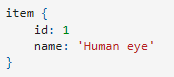
\includegraphics[scale=1]{ReteNeurale/EyeDetection/Dataset/Images/eyelabelmap_item.png}
    \caption{Eye Detection labelmap.pbtxt}
    \label{fig:eyelabelmap}
\end{figure}

\subsection{Trainig}
\label{sub:gazetraining}
Si è quindi proceduto all’addestramento della rete tramite Python usando TensorFlow e le API di Keras. Si è reso necessario modificare il file \textit{pipeline.config} adattandolo alle nostre esigenze:

\begin{itemize}
    \item \textit{numclasses} che corrisponde al numero di item da identificare;
    \item \textit{path} vari da adattare al nostro workspace, tra cui il path per i checkpoint, per i record di input e per il labelmap.
\end{itemize}

Durante il procedimento di training si sono tenuti controllati i valori della nostra rete. In particolare, abbiamo usato \textbf{Tensorboard}: un framework grafico utile a capire l'andamento della nostra rete, infatti abbiamo avuto modo di controllare ad ogni training le performance della nostra rete di machine learning.

TensorBoard fornisce la visualizzazione e gli strumenti necessari per la sperimentazione del machine learning:

\begin{itemize}
    \item Monitoraggio e visualizzazione di metriche come perdita e precisione;
    \item Visualizzazione del grafico del modello (operazioni e livelli);
    \item Visualizzazione degli istogrammi di pesi, distorsioni o altri tensori man mano che cambiano nel tempo.
\end{itemize}

\begin{figure}[htbp]
    \centering
    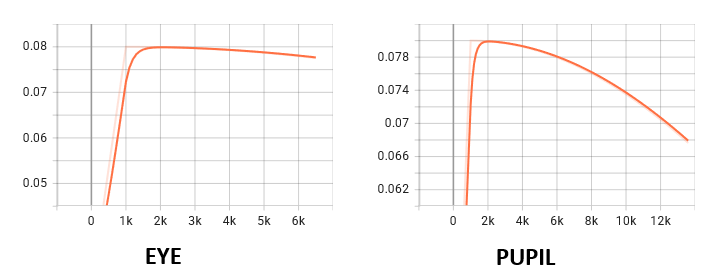
\includegraphics[scale=0.7]{ReteNeurale/EyeDetection/Training/Images/learning_rate_both_edited.png}
    \caption{Tensorboard Learning\_rate}
    \label{fig:eyelearningrate}
\end{figure}

Si è ottenuto in output un modello addestrato e pronto all’uso.

\begin{figure}[htbp]
    \centering
    \subfigure[Test personaggio famoso]{
    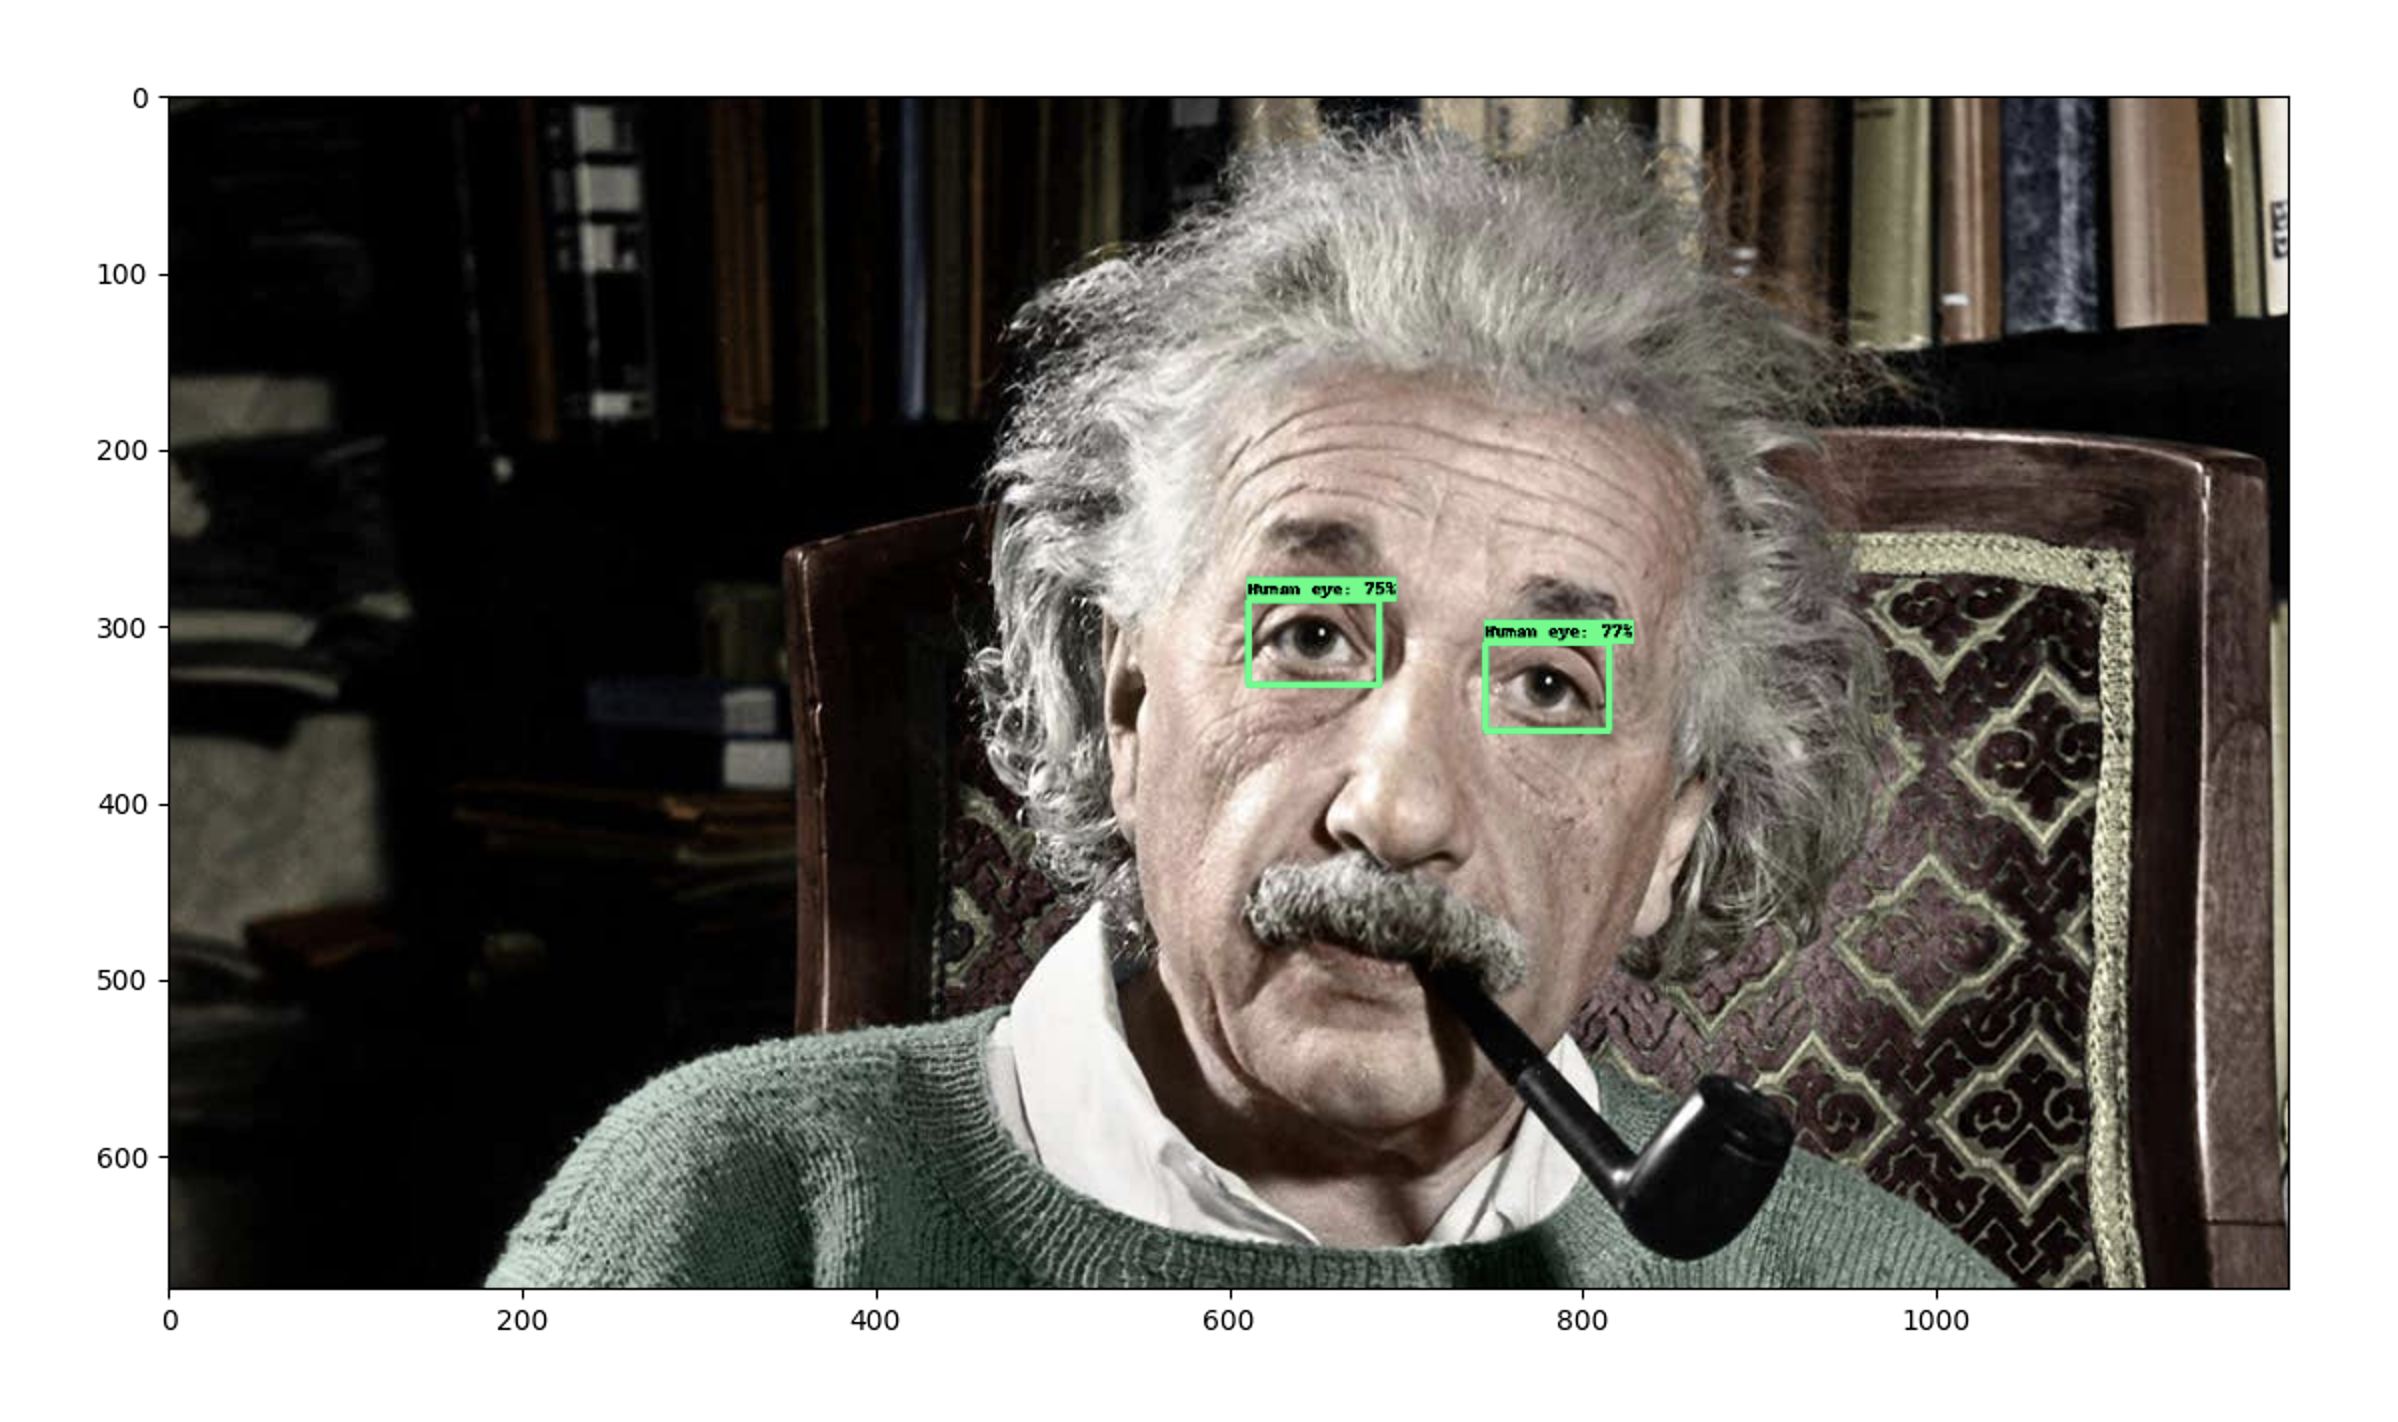
\includegraphics[scale=0.16]{ReteNeurale/EyeDetection/Training/Images/einstein.png}
    \label{fig:testeyeinstein}
    }
    \hspace{5mm}
    \subfigure[Test multiplo]{
    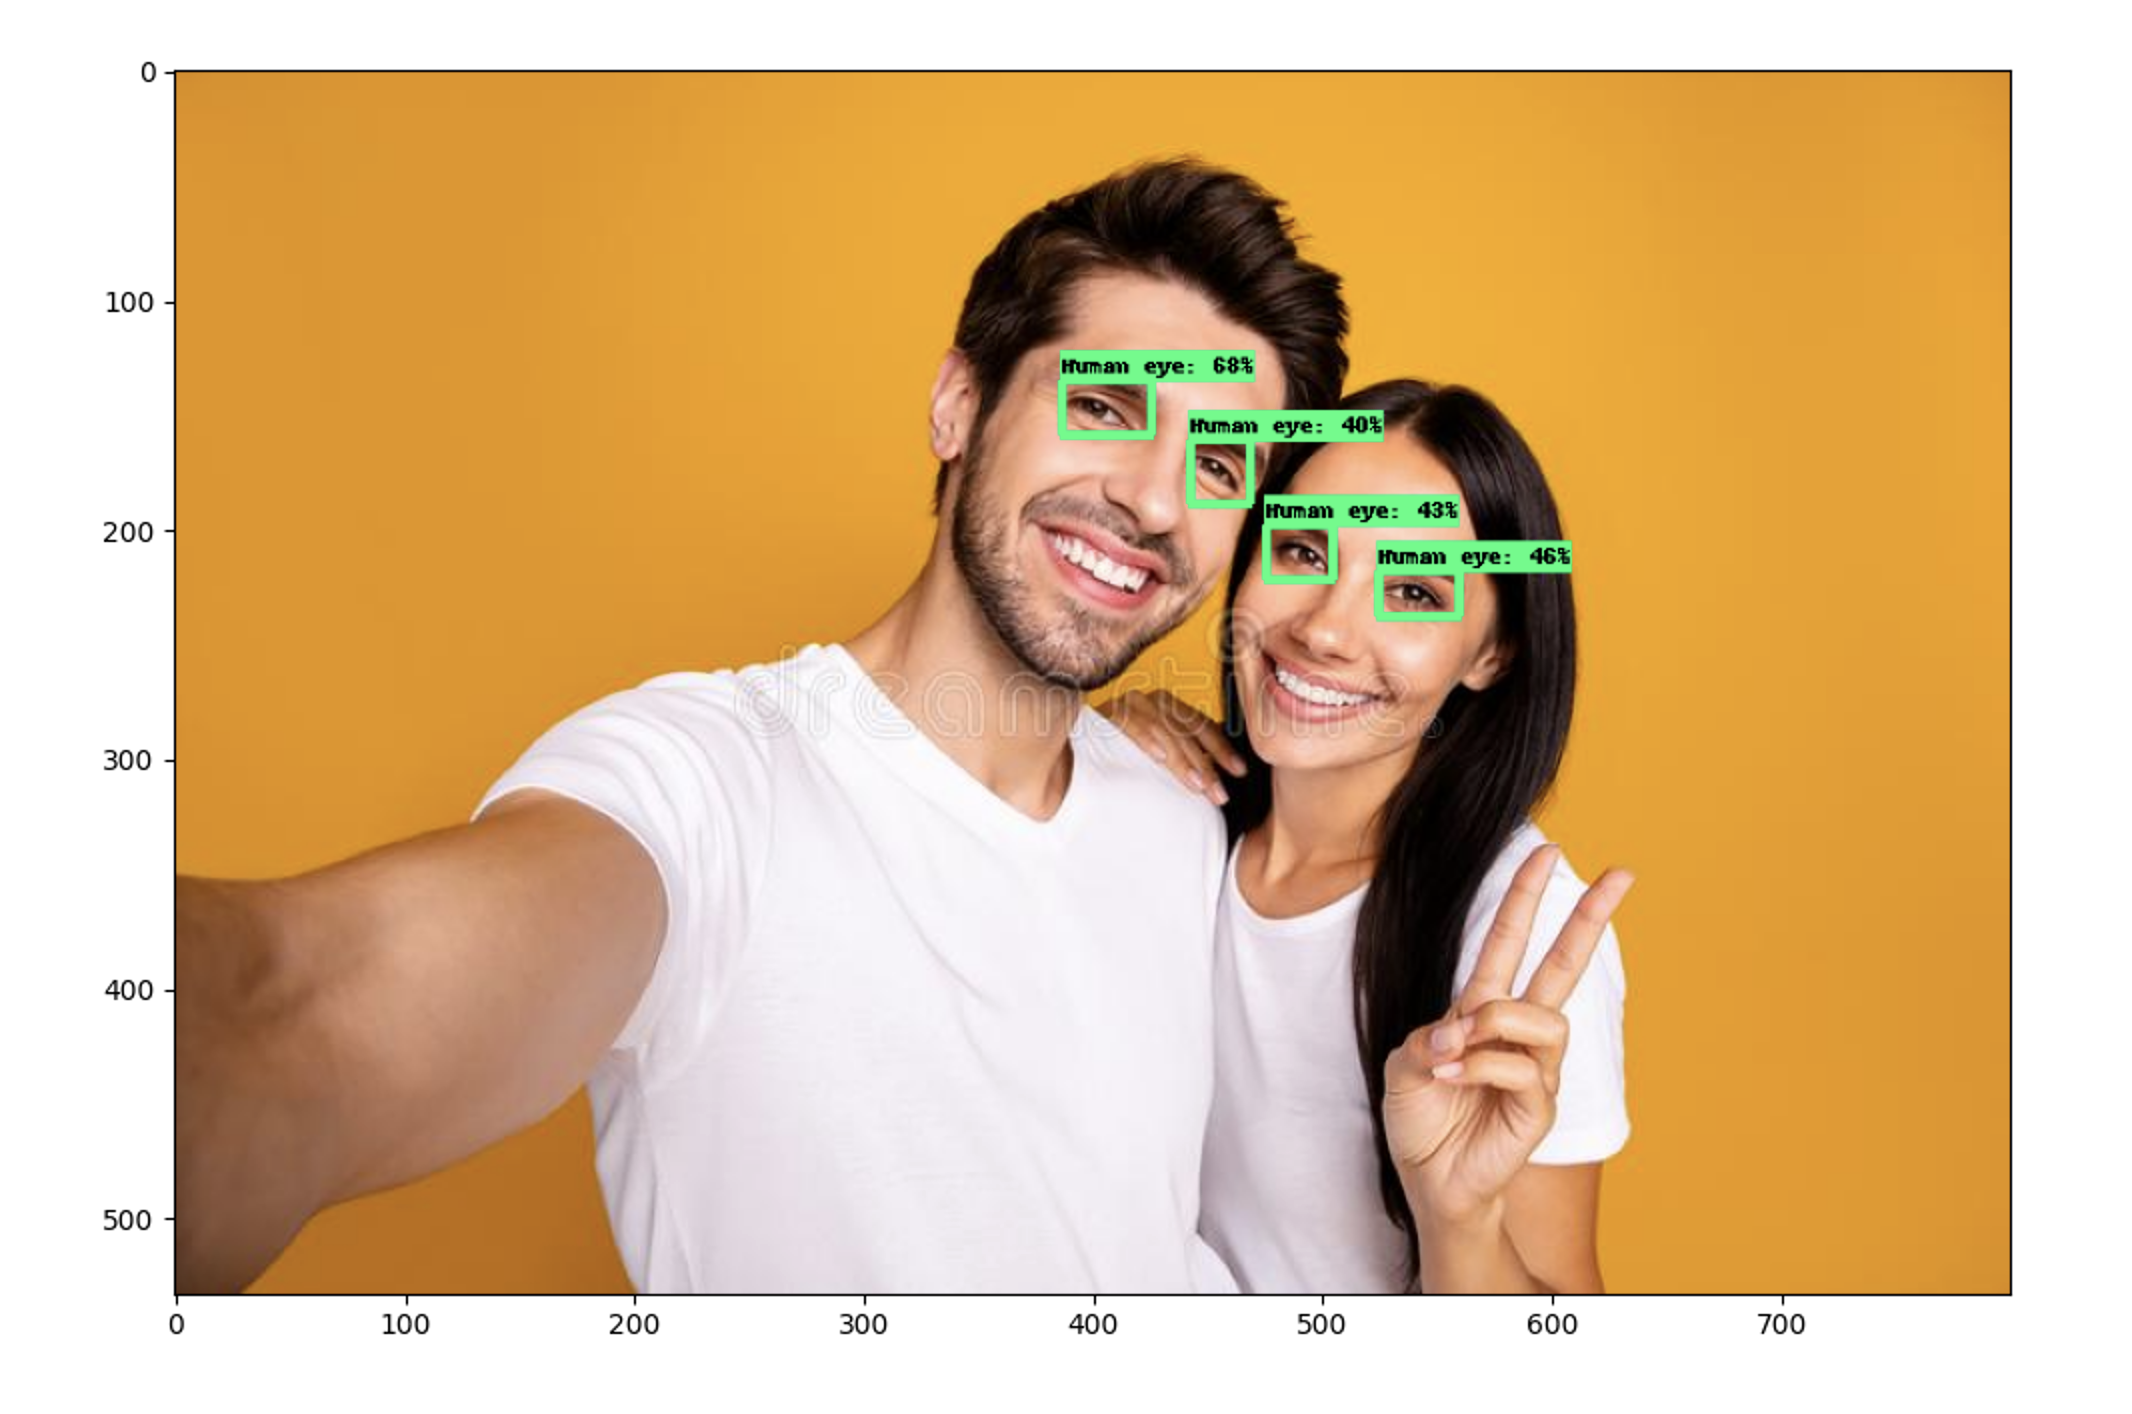
\includegraphics[scale=0.16]{ReteNeurale/EyeDetection/Training/Images/gruppo.png}
    \label{fig:testeyegruppo}
    }
    \caption{Test Eye-Tracking}
    \label{fig:testeyetracking}
\end{figure}

Prima di testare direttamente su Android, abbiamo deciso prima di testare e analizzare la nostra nuova rete utilizzando la libreria Matplotlib, utile per visualizzare graficamente via shell i nostri risultati. In particolare abbiamo usato \textbf{Tkinter}, l'unico framework GUI incluso nella libreria standard di Python.

A fini di testing si è preso ad esempio il volto di un
personaggio pubblico, quello di Albert Einstein, e anche un'immagine contenente più persone in modo tale da poter verificare la correttezza e la precisione della rete anche in condizioni più difficili.

\subsection{TfLite}
\label{sub:gazetflite}
Dopo esserci accertati che la rete funzionasse correttamente e avesse dei livelli di precisione sopra una certa soglia, si è ottenuto in output un modello addestrato e pronto all’uso, che poi è stato convertito e quantizzato in un formato adatto ai sistemi embedded, quello di TensorFlow Lite.

\subsection{Metadata}
\label{sub:gazemetadata}
Per un corretto funzionamento della rete neurale all'interno di Android, TfLite richiede che venga generato anche un file Metadata che contiene le informazioni necessarie per pre-processare le immagini. Questo file si rende necessario in quanto i nostri tensori di input sono di tipo kTfLiteFloat32. È necessario creare un nuovo \textit{label\_map.txt} con al suo interno nella prima riga il nostro item per la detection: nel nostro caso \textit{"Human eye"}.

Una volta generato questo nuovo file metadata.tflite siamo pronti ad importarlo all'interno della nostra applicazione Android come file di Machine Learning "$ml$".